\documentclass{article}
\usepackage[utf8]{inputenc}

%\title{}
\title{%
  A qualitative comparison study between \\  
  common GPGPU frameworks. \\
  \large Planning Report, Rev 0.1 \\
}
\author{
    Adam Söderström 930327-3750 \\
    adaso578@student.liu.se 
}
\date{January 2018}

\usepackage{natbib}
\usepackage{graphicx}
\usepackage{rotating}
\usepackage{subcaption}

\begin{document}
\maketitle

\section{Background}
The performance inclination of single-cored CPU's have during the last decades slowly started to decline. The main reason for this declination is due to three walls:

\begin{itemize}
    \item Instruction Level parallelism wall --- not enough instruction level parallelism to keep the CPU busy
    \item Memory wall --- gap between the CPU speed and off-chip memory
    \item Power wall --- Increased clock rate needs more power which leads to heat problems
\end{itemize}

\noindent This has started a trend where Central Processing Unit (CPU) manufactures have started to create chips containing multiple cores that are run in parallel, see figure \ref{fig:cpuStats}. Today modern CPU's may contain as much as 24 cores, and the number of cores available on a chip seem to be increasing. This technology is however already in use in Graphical Processing Units (GPU), which may contain hundreds of cores. This in turn have spawned a new trend among developers to not just use the GPU to render graphics to the screen, but to perform more general computations. The term used for this is General-purpose computing on graphics processing units (GPGPU).

\begin{figure}[!h]
    \centering
    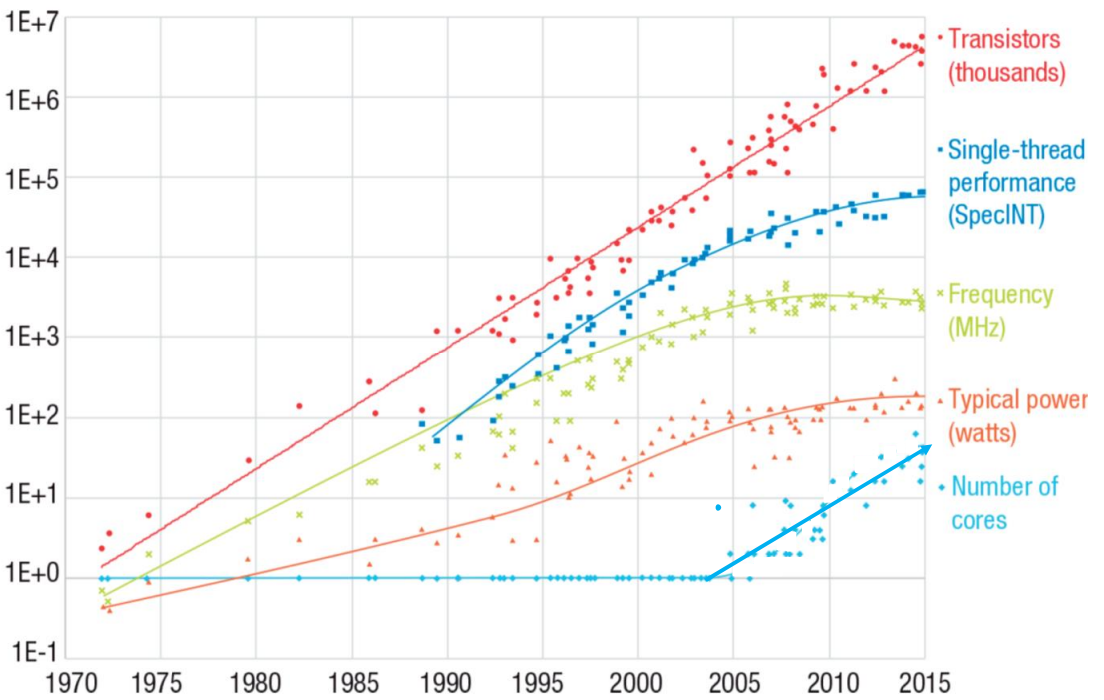
\includegraphics[width=12cm]{Figs/CPUStats.png}
    \caption{Statistics of development for CPU's. \cite{CPUStats}}
    \label{fig:cpuStats}
\end{figure}

In 2007, Nvidia released their framework called CUDA which was developed specifically for GPGPU. Since then, more frameworks and platforms have emerged, most noticeably Open Computing Language (OpenCL), Microsoft's Compute Shaders for DirectX called DirectCompute and OpenGL's version of compute shaders. This thesis will focus on evaluating GPGPU frameworks as well as a SkePU implementation when running a suitable algorithm in terms of performance, portability and features. The thesis will be performed at the company MindRoad AB.

\subsection{Algorithm} \label{subsec:algorithm}
This section will discuss algorithms that are candidates for implementation and evaluation. A short description of the algorithm will be presented along with why the algorithm is suitable for a bench-marking application.

\subsubsection{N-body}
An N-Body simulation is an interesting implementation that can be well parallelized. A $N$ number of bodies are simulated where each body is affected by forces from all other bodies. The traditional implementation does thus run in the time complexity $O(n^2)$ but can be further optimized by using the Barnes-Hut algorithm which uses an quad/octree the reduce the time complexity to $O(n \ log \ n)$ \cite{barnes1986hierarchical}. An N-body simulation is often used in traditional GPU bench-marking tests, and it would be interesting to investigate this further when implemented using a GPGPU approach. The bench-marking can be performed in multiple ways; in a real-time simulation and compare the frames-per-second (FPS) with the size of N. In a pre-computed simulation for a fixed amount of time-steps $t_n$, the bench-marking can be performed by comparing the computation time for the entire time-space.

\vspace{5mm}
\noindent \textbf{Relevant litterature:}
\begin{itemize}
    \item Barnes, J. and Hut, P., 1986. A hierarchical O (N log N) force-calculation algorithm. nature, 324(6096), p.446. \cite{barnes1986hierarchical}
    \item Burtscher, M. and Pingali, K., 2011. An efficient CUDA implementation of the tree-based barnes hut n-body algorithm. GPU computing Gems Emerald edition, 75. \cite{burtscher2011efficient}
    \item Aarseth, S.J. and Aarseth, S.J., 2003. Gravitational N-body simulations: tools and algorithms. Cambridge University Press. \cite{aarseth2003gravitational}
    \item Hamada, T., Nitadori, K., Benkrid, K., Ohno, Y., Morimoto, G., Masada, T., Shibata, Y., Oguri, K. and Taiji, M., 2009. A novel multiple-walk parallel algorithm for the Barnes–Hut treecode on GPUs–towards cost effective, high performance N-body simulation. Computer science-research and development, 24(1), pp.21-31. \cite{hamada2009novel}
    \item Singh, J.P., Holt, C., Totsuka, T., Gupta, A. and Hennessy, J., 1995. Load balancing and data locality in adaptive hierarchical N-body methods: Barnes-Hut, fast multipole, and radiosity. Journal of Parallel and Distributed Computing, 27(2), pp.118-141. \cite{singh1995load}
    \item Nyland, L., Harris, M. and Prins, J., 2007. Fast n-body simulation with cuda. GPU gems, 3(31), pp.677-695. \cite{nyland2007fast}
\end{itemize}

\subsubsection{Parallel Quick-Sort}
The quick-sort algorithm is one of the most popular sorting algorithms. The sorting algorithm runs in the time complexity  $O(n \ log \ n)$ in average, and in the worst case  $O(n^2)$. Although a very popular sequential algorithm, it is not as popular in parallel applications due to its data dependent reorganization. Some research has been done on the subject though and parallel implementations exists \cite{sanders1997efficient}\cite{tsigas2003simple}\cite{manca2016cuda}. The bench-marking in this algorithm can be done by comparing the time consumption when sorting the same input data for all relevant frameworks.

\vspace{5mm}
\noindent \textbf{Relevant litterature:}
\begin{itemize}
    \item Hoare, C.A., 1962. Quicksort. The Computer Journal, 5(1), pp.10-16. \cite{hoare1962quicksort}
    \item Sanders, P. and Hansch, T., 1997, June. Efficient massively parallel quicksort. In International Symposium on Solving Irregularly Structured Problems in Parallel (pp. 13-24). Springer, Berlin, Heidelberg. \cite{sanders1997efficient}
    \item Manca, E., Manconi, A., Orro, A., Armano, G. and Milanesi, L., 2016. CUDA‐quicksort: an improved GPU‐based implementation of quicksort. Concurrency and Computation: Practice and Experience, 28(1), pp.21-43. \cite{manca2016cuda}
\end{itemize}

\subsubsection{Anti Aliasing using an Euclidean distance transform function}
A problem in computer graphics is the inability to render sharp surface features when rendered up close, sharp edges in textures often appear jagged when rendered up close. In 2007, Chris Green of Valve Software published a method of dealing with this problem by generating a distance function for a binary image \cite{green2007improved}. An example of C. Green's method applied to a  alpha-blended texture can be seen in figure \ref{fig:valve} \cite{green2007improved}. S. Gustavson et. al. later released an improved version of C. Green's idea, which uses an euclidean distance transform (DT) \cite{gustavson2011anti}\cite{gustavson20122d}. 


\begin{figure}[!h]
    \centering
    \begin{subfigure}[b]{0.271\textwidth}
        
\includegraphics[width=\textwidth]{Figs/ValveAlphaBlended.png}
        \caption{64x64 texture, alpha-blended}
        \label{fig:valveA}
    \end{subfigure}
    ~
    \begin{subfigure}[b]{0.3\textwidth}
        
\includegraphics[width=\textwidth]{Figs/ValveAlphaTested.png}
        \caption{64x64 texture, alpha tested}
        \label{fig:valveA}
    \end{subfigure}
    ~ 
    \begin{subfigure}[b]{0.3\textwidth}
        
\includegraphics[width=\textwidth]{Figs/ValveGreensTechnique.png}
        \caption{64x64 texture using Green's technique}
        \label{fig:mouse}
    \end{subfigure}
    \caption{Vector art encoded in a 64x64 texture using (a) simple bilinear filtering (b) alpha testing and (c) Green's distance field technique}\label{fig:animals}
    \label{fig:valve}
\end{figure}

V. Ilic et. al. later extended this into three-dimensions using a similar DT technique based on C. Green's technique \cite{ilic2015precise}. 

The algorithm works on pixel level and is thus very well suitable for parallelization. It is also easy to use this algorithm for a bench-mark application by comparing the time consumption when running the algorithm on the different frameworks.


\vspace{5mm}
\noindent \textbf{Relevant litterature:}
\begin{itemize}
    \item Green, C., 2007, August. Improved alpha-tested magnification for vector textures and special effects. In ACM SIGGRAPH 2007 courses (pp. 9-18). ACM. \cite{green2007improved}
    \item Gustavson, S. and Strand, R., 2011. Anti-aliased Euclidean distance transform. Pattern Recognition Letters, 32(2), pp.252-257. \cite{gustavson2011anti}
    \item Gustavson, S., 2012. 2D shape rendering by distance fields. \cite{gustavson20122d}
    \item Ilić, V., Lindblad, J. and Sladoje, N., 2015. Precise Euclidean distance transforms in 3D from voxel coverage representation. Pattern Recognition Letters, 65, pp.184-191. \cite{ilic2015precise}
\end{itemize}

\subsection{Selected algorithm}
After a preliminary study has been made, the N-Body problem will be implemented in this thesis work, optimized by using the Barnes-Hut algorithm \cite{barnes1986hierarchical}. The reason this algorithm was chosen is because of its well parallelizable nature, as well as a problem being complex enough to be implemented in the discussed frameworks in the given time frame.

\section{Problem formulation}
\begin{itemize}
    \item What is a suitable bench-marking algorithm?
    \item What factors can be compared more than the execution time?
    \item How does a parallel implementation compare to a sequential implementation?
\end{itemize}


\section{Approach}
The report will be written in parallel with the implementation and will written according to the Gantt-chart presented in figure \ref{fig:GanttChart}. The Gantt-chart also specifies more precise time approximations and scheduling.

At the end of each week a short summary describing the work performed will be submitted to the examiner and to MindRoad AB.

\begin{itemize}
    \item Explore previous comparisons/benchmarks between CUDA, OpenCL and DirectCompute. 
    \item Investigate the algorithm and find parts that can be parallelized.
    \item Examine previous research on the subject.
    \item Investigate useful technologies that can be used in the implementation.
    \item Implement a simple "Hello World" application in all environments.
    \item Develop a sequential implementation used for comparison.
    \item Implement a CUDA application running the algorithm, perform necessary optimization's.
    \item Port the CUDA implementation to OpenCL and DirectCompute.
    \item Perform measurements between the different implementations.
\end{itemize}


\begin{sidewaysfigure}[!h]
    \centering
    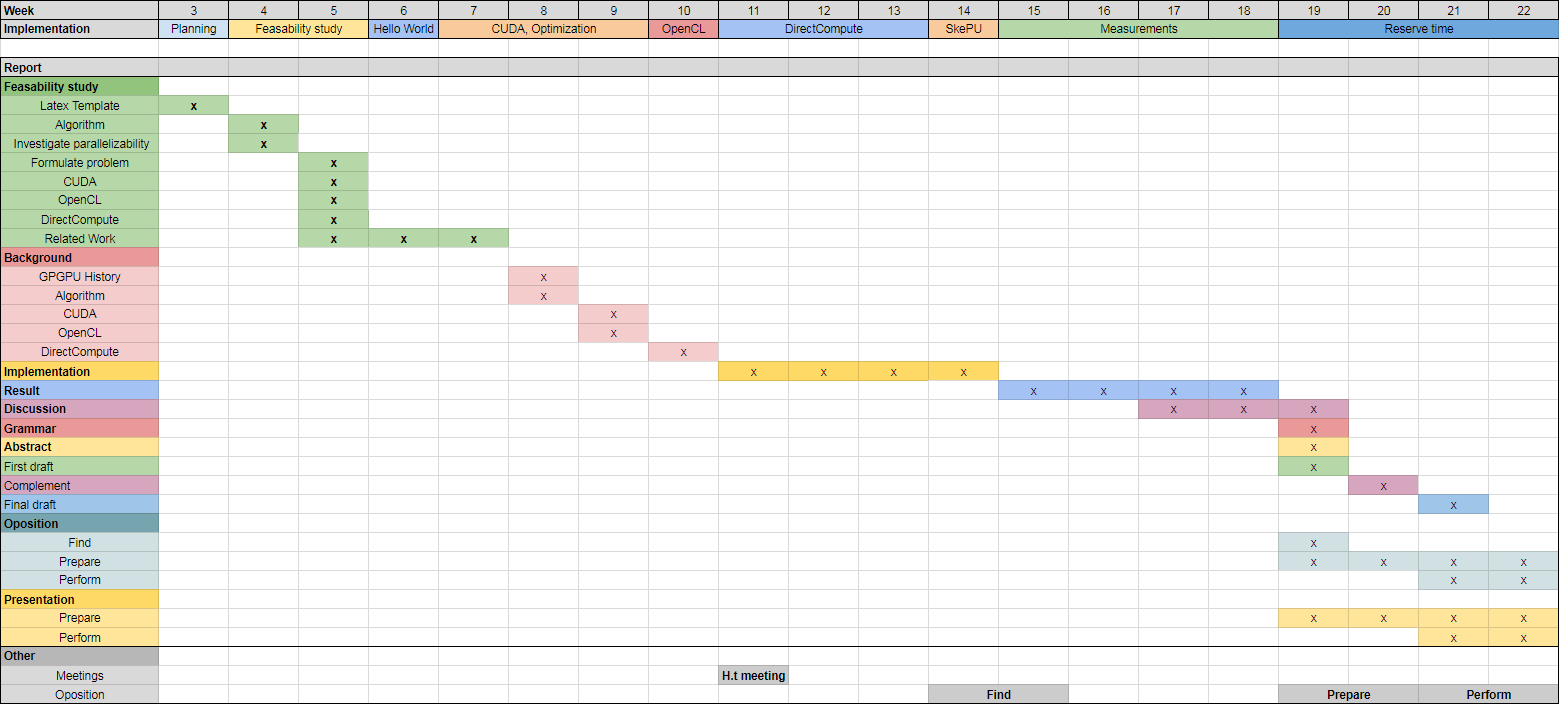
\includegraphics[width=1.1\textwidth]{Figs/Gantt-chart.png}
    \caption{Detailed Gantt-chart describing the implementation and report work-flow}
    \label{fig:GanttChart}
\end{sidewaysfigure}




\section{Delimitations}
This section will present some delimitations for the implementation and evaluation.

The selected algorithm will only be implemented in the discussed frameworks:
\begin{itemize}
    \item CUDA
    \item OpenCL
    \item DirectCompute
\end{itemize}

\noindent aswell as an implementation in SkePU, running OpenCL, CUDA, OpenMP and a sequential backend \cite{enmyren2010skepu}. The selected algorithm will thus not be implemented in other GPGPU frameworks such as OpenGL's compute shader, or a parallel CPU based implementation, using e.g OpenMP or similar frameworks.

Even though other optimization algorithms exists for the N-Body problem, only the Barnes-Hut algorithm will be implemented in this work. The reason for this is because the thesis will not focus on evaluating the performance of the algorithm, but on the comparison between frameworks which multiple optimization techniques implementations won't contribute to. Furthermore to give the implementation a fair comparison, the tree-structure used in Barnes-Hut will be a sequential implementation and performed on the host.

\section{Resources}

Below follows a list of resources used in this thesis work:

\begin{itemize}
    \item CUDA - http://docs.nvidia.com/cuda/
    \item OpenCL - https://www.khronos.org/opencl/
    \item DirectCompute - https://msdn.microsoft.com/en-us/library/windows/desktop/ff476331(v=vs.85).aspx
    \item SkePU - http://www.ida.liu.se/labs/pelab/skepu/
    \item Course material from the course TDDD56 - Multicore and GPU Programming 
\end{itemize}


\bibliographystyle{plain}
\bibliography{references}

\end{document}
